\documentclass{article}
\usepackage{amsmath}
\usepackage{graphicx} 
\usepackage{xcolor}
\usepackage{listings}
\usepackage{hyperref}
\usepackage{cleveref}
\usepackage{geometry}
\usepackage{enumitem}

\usepackage{tikz}
\usepackage{pgfplots}
\usepackage{circuitikz}

\title{Test Title}
\author{Dan Lynch}
\date{v0.0.1 January 2025}

\begin{document}

\maketitle

\tableofcontents

\section{Introduction}

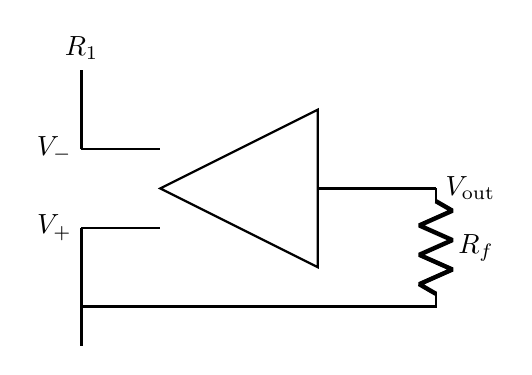
\begin{tikzpicture}
  % Draw the op-amp triangle
  \draw[thick] (0,0) -- (2,1) -- (2,-1) -- cycle;
  
  % Draw and label the inverting input (-)
  \draw[thick] (-1,0.5) -- (0,0.5);
  \node[left] at (-1,0.5) {$V_-$};
  \draw[thick] (-1,0.5) -- (-1,1.5) node[above] {$R_1$};
  
  % Draw and label the non-inverting input (+)
  \draw[thick] (-1,-0.5) -- (0,-0.5);
  \node[left] at (-1,-0.5) {$V_+$};
  
  % Output
  \draw[thick] (2,0) -- (3.5,0);
  \node[right] at (3.5,0) {$V_{\text{out}}$};
  
  % Feedback loop
  \draw[thick] (3.5,0) to[R, l=$R_f$] (3.5,-1.5) -- (-1,-1.5) -- (-1,-0.5);
  
  % Ground for non-inverting input
  \draw[thick] (-1,-1.5) to[ground] (-1,-2);
\end{tikzpicture}


\end{document}